\documentclass[a4paper,12pt]{article}

\usepackage[utf8]{inputenc}
\usepackage[T1]{fontenc} % serif: fontenc, palatino, fouriernc, lmodern
\usepackage{fullpage}
\usepackage{amsfonts, amsmath, amssymb, amstext, latexsym, stmaryrd, ulem}
\usepackage{graphicx, epsfig, wrapfig, exscale, amsbsy, amsopn, fancyhdr}
\usepackage{subfigure, xspace, enumerate, caption, mathrsfs, pdfpages}
\usepackage{url, tikz}
\usetikzlibrary{positioning, arrows}


\begin{document}

\begin{center}
{\fontsize{20pt}{20pt} \selectfont \textbf{Chinese Restaurant Process Collocations}}
\vskip 10pt
Gabriel Synnaeve, Benjamin B\"{o}rschinger
\vskip 10pt
\hrule height 4pt
\end{center}

This presents a model for unsupervised word segmentation, that does no linguistic assumption at all.

\section{CRP Model}

%%% TODO

\section{Equivalent Adaptor Grammar}
\begin{eqnarray}
    Root & \rightarrow & Levels_N\\
    Levels_N & \rightarrow & Level_N\ Levels_N\\
    \underline{Level_N} & \rightarrow & Levels_{N-1}\\
    Levels_{N-1} & \rightarrow & Level_{N-1}\ Levels_{N-1}\\
    & \dots & \\
    Levels_1 & \rightarrow & Level_1\ Levels_1\\
    \underline{Level_1} & \rightarrow & Phones\\
    Phones & \rightarrow & Phon\ Phones\\
    Phon & \rightarrow & terminal
\end{eqnarray}

\section{Example}

Let us consider the sentence ``the dog barks'' with the following segmentation:\\
\begin{small}
\texttt{(L3 (L2 (L1 the) (L1 dog) ) (L2 (L1 barks) (L1 at) ) (L2 (L1 the) (L1 cat) ) )}
\end{small}

If there was only this sentence in the dataset, we would get Figure~\ref{fig:HCRP1}.

\begin{figure}
\centering

\begin{scriptsize}
\begin{subfigure}[The $L3$ restaurant has only one table.]{
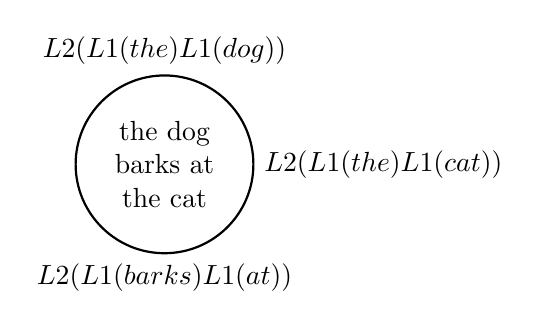
\begin{tikzpicture} 
\node [circle,thick,draw,align=center,
label={[black]above:$L2(L1(the) L1(dog))$},
label={[black]below:$L2(L1(barks) L1(at))$},
label={[black]right:$L2(L1(the) L1(cat))$},
text width=1.6cm,
] {the dog barks at the cat};
\end{tikzpicture}}
\end{subfigure}

\begin{subfigure}[The $L2$ restaurant has 3 tables.]{
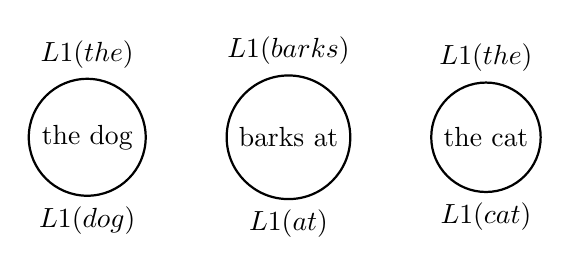
\begin{tikzpicture}
\node [circle,thick,draw,
label={[black]above:$L1(the)$},
label={[black]below:$L1(dog)$},
] (t1) {the dog};
\node [circle,thick,draw,
label={[black]above:$L1(barks)$},
label={[black]below:$L1(at)$},
] (t2) [right=of t1] {barks at};
\node [circle,thick,draw,
label={[black]above:$L1(the)$},
label={[black]below:$L1(cat)$},
] (t3) [right=of t2] {the cat};
\end{tikzpicture}}
\end{subfigure}

\begin{subfigure}[The $L1$ restaurant has 5 tables.]{
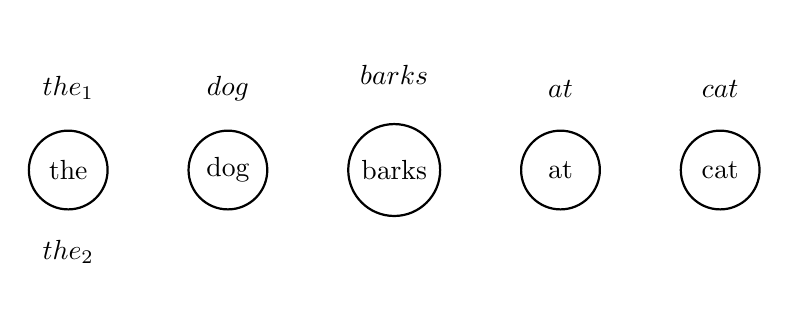
\begin{tikzpicture}[every node/.style={circle,draw,thick,minimum size=1cm}]
\node [
label={[black]above:$the_1$},
label={[black]below:$the_2$},
] (t1) {the};
\node [
label={[black]above:$dog$},
] (t2) [right=of t1] {dog};
\node [
label={[black]above:$barks$},
] (t3) [right=of t2] {barks};
\node [
label={[black]above:$at$},
] (t4) [right=of t3] {at};
\node [
label={[black]above:$cat$},
] (t5) [right=of t4] {cat};
\end{tikzpicture}}
\end{subfigure}
\end{scriptsize}
\caption{The 3 restaurants for all 3 levels.}
\label{fig:HCRP1}

\end{figure}




\end{document}
